%!TEX root =  ../final-report.tex

% Chapters are setup to start on a new page.
% The short version of that title appears in square brackets. This is used for the table of contents listing. 
% The long version of the title has a command "\setstretch{0.5}" in order to reduce the line spacing in the
% title and then the title text.
\chapter{E-field Antenna}
\label{sec:E-field Antenna}

% Sections will automatically be numbered by LaTeX. 
\section{Background}

The data acquisition system of a grain bin is based on the use of microwave imaging system to estimate the dielectric properties of the material in the grain bin. As explained in the section of introduction. The object of the antenna is to receive or transmit scattering parameter data to local PC for analyzing propose.

\begin{table}[h]
\centering
\caption{specification of the E-filed antenna}
\label{efield antenna specs}
\begin{tabular}{|l|l|}
\hline
Specifications                                   & Value              \\ \hline
Resonant frequency                               & 70MHz - 90MHz      \\ \hline
$S_{11}$ at operating frequency                       & Below -6dB         \\ \hline
Antenna size                                     & Maximum 10 $\times$ 15 cm \\ \hline
Co-plane and cross-plane polarization difference & At least 15dB      \\ \hline
Number of antennas in an array                   & 24                 \\ \hline
\end{tabular}
\end{table}

In the previous MWI system, the straight line monopole antenna with a total length of 1m is used inside the bin, however, in the resonant chamber each antenna size cannot exceed a 10*15 cm due to the volume limitation of the inner space. After investigating several options focusing on classes of small patch antennas, a suitable and feasible method has come up as meandered monopole antenna printed on a PCB layer. The FR4 with  = 4.4 will be used as the dielectric substrate of the PCB board.

\section{Research and Design}

We will start the design process from the researching and simulating the features of the simple straight line monopole antenna, then we need to determine the parameters of the meandered antenna in order to increase numbers of meandered sections to satisfy the size requirement.

The following parameters we need to consider:

\begin{itemize*}

  \item Numbers of meander sections
  \item Spacing of meander sections
  \item Bending angles for each section

\end{itemize*}

A simple single straight line monopole antenna can be represented using an equivalent inductor circuit model in Fig .1. If an additional equivalent component is added up to the self-inductance of the antenna, the resonant frequency of the meander line will be relatively change compared with previous antenna with same height, this method will provide us a reasonable approximation of the working principle of this class of antenna.

Next we need to demonstrate several simulations and optimizations to figure out how the meander line configurations will change the performance of the antenna return loss curve (S11), radiation patterns in terms of the parameters given above. In these cases, it is predicted that the inductor circuit model will not be adequate for explaining the relative changes of the resonant frequencies.[3]

\begin{figure}[h]
	\begin{center}
		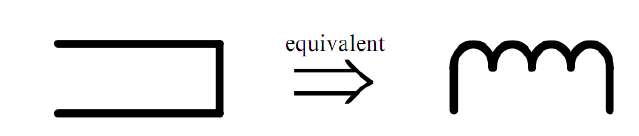
\includegraphics[width=3.8in]{./images/efield_image1.png}
		\caption{}
		\label{fig:efield_fig1}
	\end{center}
\end{figure}


Since the self-resonant frequency of the simple straight line monopole antenna can be modeled as the inductor circuit model, we can use the formula \eqref{eq1} to calculate the self-inductance when the total physical length of the antenna is about $\lambda/4$. 

\begin{equation}\label{eq1}Ls = 0.2384 λ (ln 4) \end{equation}

Where d is the diameter of the radiator of the antenna and $\lambda$ is the required resonant wavelength, the resonant frequency of the antenna can be estimated using an inductor circuit model representation as introduced in figure \ref{fig:efield_fig1}. To determine the inductance in each meandered section, we will use an equivalent transmission line model which has a characteristic impedance given as 276log(2), where s is the spacing between each meandered section, as a result, the equivalent inductance of each section, Lm, is given as following:

\begin{equation}\label{eq2}Lm =  \end{equation}

Where  is the propagation factor of free space, l is the length of each meandered section and is angular velocity, the resonant frequency of the meandered line antenna should have same physical length as the simple straight line monopole antenna, but we need to replace the equivalent inductor Ls by the sum of Ls+NLm, where N is the number of meander sections.

In order to exam the resonant behavior of the meandered line antenna, we will simulate and use optimism method in HFSS to compare each group of meandered antenna parameters given above. M0 to M5 configurations shown in figure \ref{fig:efield_fig2} (Best, Morrow) is applied to observe the variation the resonant frequency of the antenna.[1],[2]

\begin{figure}[h]
	\begin{center}
		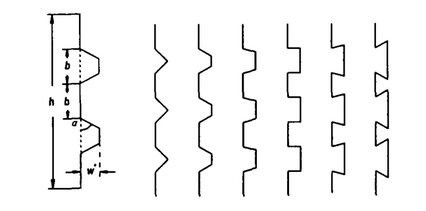
\includegraphics[width=3.8in]{./images/efield_image2.png}
		\caption{meandered monopole antenna geometry}
		\label{fig:efield_fig2}
	\end{center}
\end{figure}

The M0 configuration has a self-resonant frequency at 80MHZ, while the M5 configuration has a self-resonant frequency at 110MHZ. For antenna represented in Fig 1, s is equal to 1cm, L is equal to 4cm, using equation (2) and (3), and the value of Lm is calculated as about 300nH, a comparison table of resonant behavior of different numbers of section is listed in figure \ref{fig:efield_fig3}.

\begin{figure}[h]
	\begin{center}
		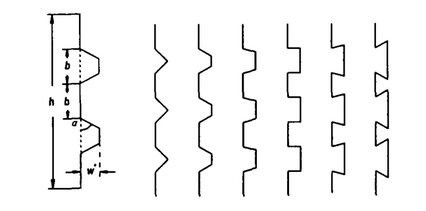
\includegraphics[width=3.8in]{./images/efield_image2.png}
		\caption{meandered monopole antenna geometry}
		\label{fig:efield_fig3}
	\end{center}
\end{figure}

From figure \ref{fig:efield_fig3}, it is evident that the inductor circuit model representing the meandered antenna provides an acceptable prediction showing a liner increase in resonant frequency as a function of increasing bending sections, however, in the real case, the resonant frequency of the meander line antenna will not linearly increase with the number of sections.[1],[2]

The limitation of inductor circuit model of the meandered antenna is still in examining, we simulated that some of the physical properties varied and the corresponding change of the resonant frequency. Firstly, we change the s in M1 configuration from 1cm to 2cm, the resonant frequency behavior of the antenna versus the meandered sections is shown in figure \ref{fig:efield_fig4}. We can observe that the actual resonant frequency will not precisely change as we seen in figure \ref{fig:efield_fig3}. 

\begin{figure}[h]
	\begin{center}
		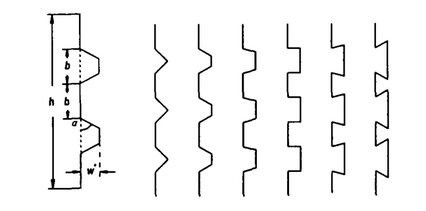
\includegraphics[width=3.8in]{./images/efield_image2.png}
		\caption{meandered monopole antenna geometry}
		\label{fig:efield_fig4}
	\end{center}
\end{figure}

Next, we examined the effect of bending angle changing for each meandered section shown in figure \ref{fig:efield_fig5} [1]

\begin{figure}[h]
	\begin{center}
		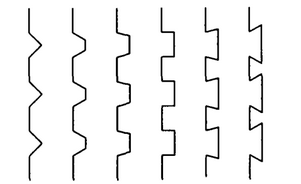
\includegraphics[width=3.8in]{./images/efield_image4.png}
		\caption{Bending angle when α= 45,60,75,90,120 degree conditions}
		\label{fig:efield_fig5}
	\end{center}
\end{figure}

We bend the antenna for the configuration M5 too see the simulation results in HFSS while keep the total physical length and spacing as the same as the previous model. The relation between bending angle and self-resonant frequency is shown in figure \ref{fig:efield_fig6}.

\begin{figure}[h]
	\begin{center}
		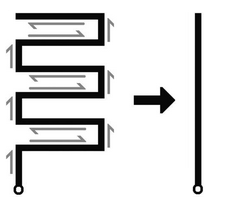
\includegraphics[width=3.8in]{./images/efield_image5.png}
		\caption{radiation principle of a 90 degrees bending meandered antenna }
		\label{fig:efield_fig6}
	\end{center}
\end{figure}

\section{Antenna building and testing}

After investigating the effects of numbers of section, section spacing and bending angle, we start to build a meandered antenna on the substrate to satisfy the specification of the antenna parameters. As seen in figure \ref{fig:efield_fig7}, the spacing between each meandered section is 0.5cm, the number of meandered sections is 14 in total, and the s11 graph is shown in figure \ref{fig:efield_fig8} which provide us a return loss below -10dB.

\begin{figure}[h]
	\begin{center}
		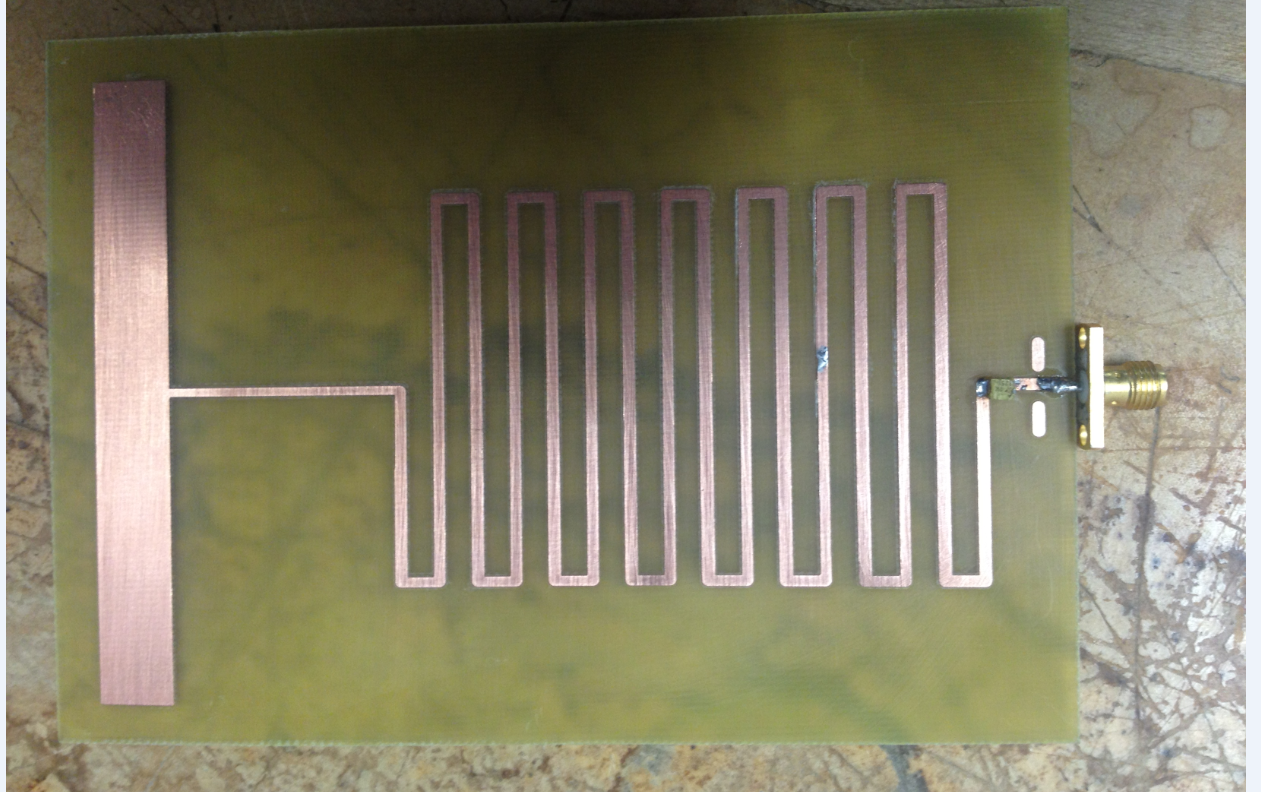
\includegraphics[width=3.8in]{./images/efield_image6.png}
		\caption{final antenna view}
		\label{fig:efield_fig7}
	\end{center}
\end{figure}

The physical length of this antenna is 80cm in total with the height of 10cm on the substrate, a top loading cap is added at the far end of the antenna to increase the s11 performance. To match up the resonant circuit, we add a 400nH inductor at the feeding point of the antenna. When testing the S12 parameter, we used a $\lambda/4$ dipole antenna as port 2 in HFSS so that the designed antenna is acting as a receiving antenna in the air box. The simulation model is shown in Fig 8. And the simulation results are listed in Fig 9-11.




\chapter{H-field Antenna}
\label{sec:H-field Antenna}

\section{Background}

Normally microwave imaging systems consist of a simple E-field antenna such and a Monopole or a Dipole antenna which has one polarization and it is limited in its functionality, however it is simple to model in software as these types of antennas produce an E-field component which is only oriented in the same direction as the antenna itself. Due to a grain storage bin being round, and closed off at both ends, it can be thought of as a cylindrical cavity resonator which has H-fields rotating around the phi direction with maximums occurring at the metallic walls of the cavity, Therefore we want to have an antenna that is capable of picking up these H-fields without picking up the E-fields that are perpendicular to the walls.

The H- field antenna design had to be confined to the following design criteria in order for it to be effective inside of the grain bin:

\begin{itemize*}

\item Ability to pick up H-field only, and reject most of the E-field
\item Minimal size (less that 15cm in length or witdth)ˆ
\item Frequency of operation between 70Mhz-90Mhzˆ
\item Matched to 50 ohm coaxial transmission lineˆ
\item Physically able to withstand grain being filled into the binˆ
\item Reduced complexity(for ease of modeling in the inversion algorithm)ˆ
\item Ease of manufacturing and reproduction

\end{itemize*}

\section{Research}

The typical design procedure for an H-field antenna is a loop of perimeter one λ as at that length the loop becomes purely resistive with the maximum amount of radiation resistance, however this approach does not work for the grain bin as the perimeter of the loop would have to be almost 4 meters.

The other typical approach to designing h-field antennas is to decrease the perimeter of the loop and increase the number of turns which allows for the required size reduction that we are looking for as well as enable it to be matched to a 50ohm coaxial line since the radiation resistance is proportional to the number of turns squared[ ], however it is also not feasible for the grain bin since it would not guarantee that the antenna does not pick up the E-field as well, and it would be too complex to model in the imaging software.

\section{Design}

In order to satisfy the main requirement of the antenna (1) a shielded and slotted loop antenna was chosen, which is a common type of antenna used in radio

\begin{figure}[h]
	\begin{center}
		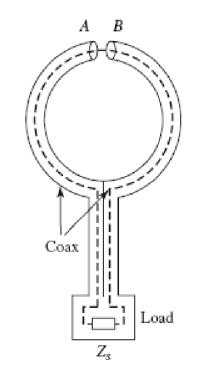
\includegraphics[width=1.5in]{./images/Figure1.jpg}
		\caption{}
		\label{fig:hfield_fig1}
	\end{center}
\end{figure}

The ground layer around the conductor which acts as the shielding modifies the electric field distribution inside of the antennas cross sectional area due to the boundary conditions on a PEC, thus reducing its effect on the antenna, this effect is confirmed in the simulation results in section [F]. Since the magnetic field passing through the loop induces a current on both the conductor and the shielding, a slot is cut out in the shield to create a capacitance which introduces a phase shift between the two currents and therefore there is a difference in potential across the load.

The second requirement (2) was met by reducing the perimeter of the antenna to $\lambda/20$, however the small size presented another challenge which is matching the loop antenna to the 50ohm coaxial line, different ways of matching were considered such as capacitive coupling and transformer coupling between the coaxial line and the antenna, These were simulated in HFSS but found the it would be too complex to build accurately, and it would not be feasible to mount in the grain bin. Mohammad (Project co-supervisor) suggested the use of a 50ohm termination at the end of the loop to match the antenna to a 50ohm line and to cut the loop in half so that the size of it could be further reduced as well as to take advantage of having a metallic wall as the other half of the loop. A prototype of this antenna was built using a semi rigid coaxial cable with a slot cut in the ground conductor and a 50 ohm termination was used to match the antenna to a coaxial line.

\begin{figure}[h]
	\begin{center}
		\includegraphics[width=4in]{./images/Figure 2.jpg}
		\caption{prototype antenna}
		\label{fig:hfield_fig2}
	\end{center}
\end{figure}

A difference of 10db was observed between the E and H polarization. However building multiples of such antennas accurately would not be feasible since the slot size would vary and produce inaccurate results as well as the curvature in the antenna is tough to reproduce accurately.

In order to make the antenna easy to manufacture and reproduce, it was decided that a PCB version would be best suitable.

\subsection{PCB Antenna Design}

To achieve a shielded coaxial line on PCB, a groundless co-planar waveguide was chosen, next after considering price as well as material availability in the lab, a 0.8mm FR-4 material was chosen as the PCB material with a relative permittivity of 4.3. Due to the limited capabilities of the PCB prototyping machine available at the EIL lab, in order to have the most accurate results a minimum cut in the PCB could not exceed 0.2mm, therefore 0.2mm was chosen as the gap between the conductor and the ground planes of the co-planar waveguide. With the help of TX-line (transmission line calculation software) a conductor size of 2.57mm with a gap of 0.2mm and a 0.8mm FR-4 thickness yields the necessary 50ohm transmission line.

\subsection{PCB Antenna Simulation}

The PCB version of the antenna is constructed in the high frequency structure simulator with FR-4 as the substrate material, copper material on top of the substrate is simulated as perfect conductor and an infinite ground plane as the antennas backing plate. The design is simulated and optimized to obtain its performance characteristics. From optimization a slot size of 1 mm is chosen in the shielding.

\begin{figure}[h]
	\begin{center}
		\includegraphics[width=4in]{./images/Figure 3.jpg}
		\caption{HFSS model}
		\label{fig:hfield_fig3}
	\end{center}
\end{figure}

\subsection{Simulation Results}

The desired result is to have an S11 (insertion loss) of -10db at the frequency of operation, and as expected the insertion loss at 80 MHz is -14.5db as well as due to the 50 ohm termination the antenna has a really high bandwidth.

The simulation also confirms the effect of the co-planar ground plane on the Electric fields inside the cross sectional area of the antenna, Figure 6 and Figure 7 show the antenna with shielding and antenna without shielding E-field magnitude distribution in the cross sectional area.

\begin{figure}[h]
	\begin{center}
		\includegraphics[width=4in]{./images/Figure 4.jpg}
		\caption{S11}
		\label{fig:hfield_fig4}
	\end{center}
\end{figure}

\begin{figure}[h]
	\begin{center}
		\includegraphics[width=4in]{./images/Figure 5.jpg}
		\caption{S11}
		\label{fig:hfield_fig5}
	\end{center}
\end{figure}

\begin{figure}[h]
	\begin{center}
		\includegraphics[width=4in]{./images/Figure 6.jpg}
		\caption{}
		\label{fig:hfield_fig6}
	\end{center}
\end{figure}

\begin{figure}[h]
	\begin{center}
		\includegraphics[width=4in]{./images/Figure 7.jpg}
		\caption{}
		\label{fig:hfield_fig7}
	\end{center}
\end{figure}

\subsection{PCB Layout}

After simulating the antenna in HFSS, the design was transferred to Altium which was used to create the necessary Gerber files for fabrication. The antenna was fabricated in the EIL with the use of the rapid PCB prototyping machine. 

\begin{figure}[h]
	\begin{center}
		\includegraphics[width=4in]{./images/Figure 8.jpg}
		\caption{fabricated antenna}
		\label{fig:hfield_fig8}
	\end{center}
\end{figure}

\subsection{H-field Antenna Testing}

The antenna’s ability to reject the Electric field was tested in a G-TEM cell (Transverse Electro Magnetic). The G-TEM cell creates transverse EM waves guided between a pair of plates with H orthogonal to E, the incident wave was created with a signal generator producing an 80 MHz sine wave with 0dbm power and the AUT measurements were taken with a spectrum analyzer. Two orientations of the antenna were tested in the cell, longitudinally parallel with the magnetic field (E-orientation) and perpendicular to magnetic field (H-orientation).

\subsection{G-TEM Test Results}

The noise floor of the antenna was measured at -83dbm with incident power of -13dbm.

When oriented in the E-orientation the antenna received -81dbm which is close to the noise level of the antenna, when oriented in the H-orientation the antenna received -65dbm therefore a difference of 16db exists between the two orientations which implies that the antenna is picking up only H.

\begin{figure}[h]
	\begin{center}
		\includegraphics[width=4in]{./images/Figure 9.jpg}
		\caption{E-orientation}
		\label{fig:hfield_fig9}
	\end{center}
\end{figure}

\begin{figure}[h]
	\begin{center}
		\includegraphics[width=4in]{./images/Figure 10.jpg}
		\caption{H-orientation}
		\label{fig:hfield_fig10}
	\end{center}
\end{figure}





\chapter{Multiplexer}
\label{sec:Multiplexer}

\section{Background}

The multiplexer consists of two sections; an RF switch section and a DC switch section. The RF switch provides a path for the signal to and from the VNA to the antennas, while the DC switch provides the logic necessary to set the correct path in the RF switch at the correct time. In order to collect the data required to create an image of the grain bins contents, an array of antennas needs to be connected to the VNA. Figure \ref{fig:mp_connections} shows how the multiplexer connects the VNA to the array of antennas. The VNA has two ports, one which transmits a signal and one which receives a signal. Through commands sent from the DC switch, the multiplexer is capable of connecting either of these two ports to any of the antennas in the array.

\begin{figure}[h]
	\begin{center}
		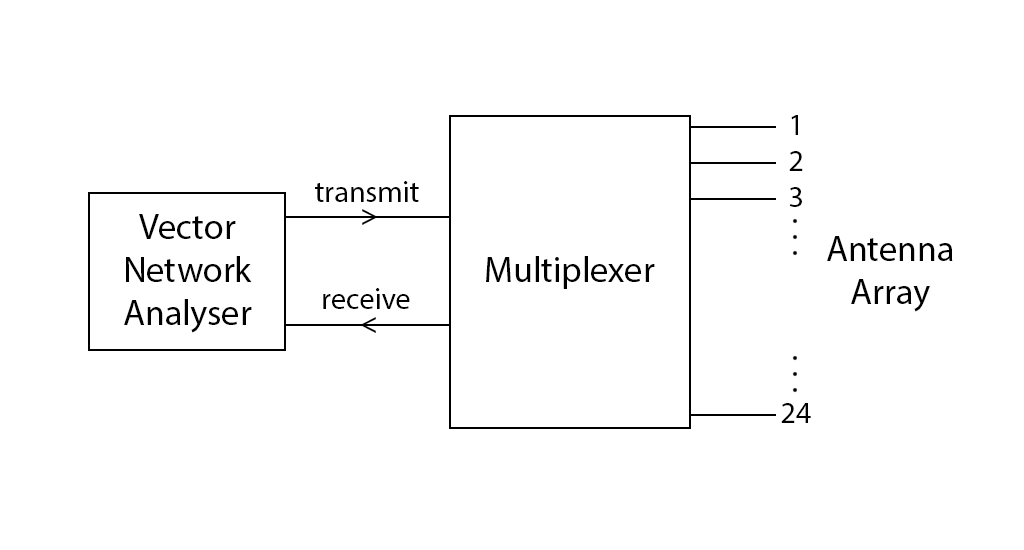
\includegraphics[width=4.5in]{./images/multiplexer_connections.png}
		\caption{Multiplexer connecting VNA to antenna array}
		\label{fig:mp_connections}
	\end{center}
\end{figure}

The multiplexer must connect the ports from the VNA in a certain sequence. First, the multiplexer will be configured to connect the transmitter port from the VNA to antenna 1. After this, antenna 2 will be connected to the receiver port of the VNA. Then antenna 3 connects to the receiver port, then antenna 4 and so on through the entire array of antennas. Once this sequence has been completed the multiplexer will now be configured to connect the transmitter port of the VNA to antenna 2, after which antenna 1 will be connected to the receiver port, then antenna 3, then antenna 4 and so on through the entire array again. The multiplexer will repeat this sequence until all antennas have acted as the transmitter with the remaining antennas acting as receivers.


\section{Design}

An initial design for the RF multiplexer was created using six 4 x 2 matrix switches together two SP3Ts. The topology of this design is shown in figure \ref{fig:mp_initial_layout}. Note that not all of the 4 x 2 matrix switches are shown in the figure, 4 more of these switches are connected to the two remaining pins of the two SP3Ts for a total of 24 antennas. The 4 x 2 matrix switch chosen for this design was from Hittite Microwave Corporation, part number HMC596LP4 and the SP3Ts chosen were part number HMC245QS16 also from Hittite Microwave Corporation.  This design was chosen for its simplicity which would allow for good performance.

However, we were not able to use this design, as it was realized that the 4 x 2 matrix switches chosen do not operate in the frequency range needed for our project of 70 - 90 MHz. More research was done but no switches of this type were found that operate in the required frequency range for this project. Due to this limitation a new design was chosen consisting of a series of cascaded RF switches, including SPDTs, SP3Ts and SP8Ts. The topology of this design is shown in figure \ref{fig:mp_final_layout}. The switches used in this design are HMC349MS8G, HMC245QS16 and HMC253QS24 from Hittite Microwave Corporation.


\begin{figure}[h]
	\begin{center}
		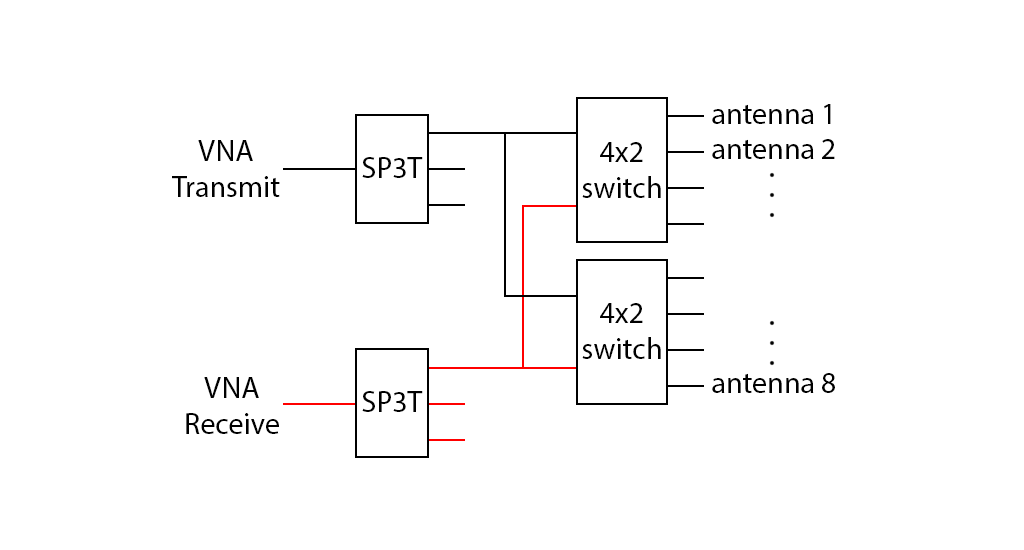
\includegraphics[width=5in]{./images/mp_initial_layout.png}
		\caption{Initial design of the multiplexer}
		\label{fig:mp_initial_layout}
	\end{center}
\end{figure}

\begin{figure}[h]
	\begin{center}
		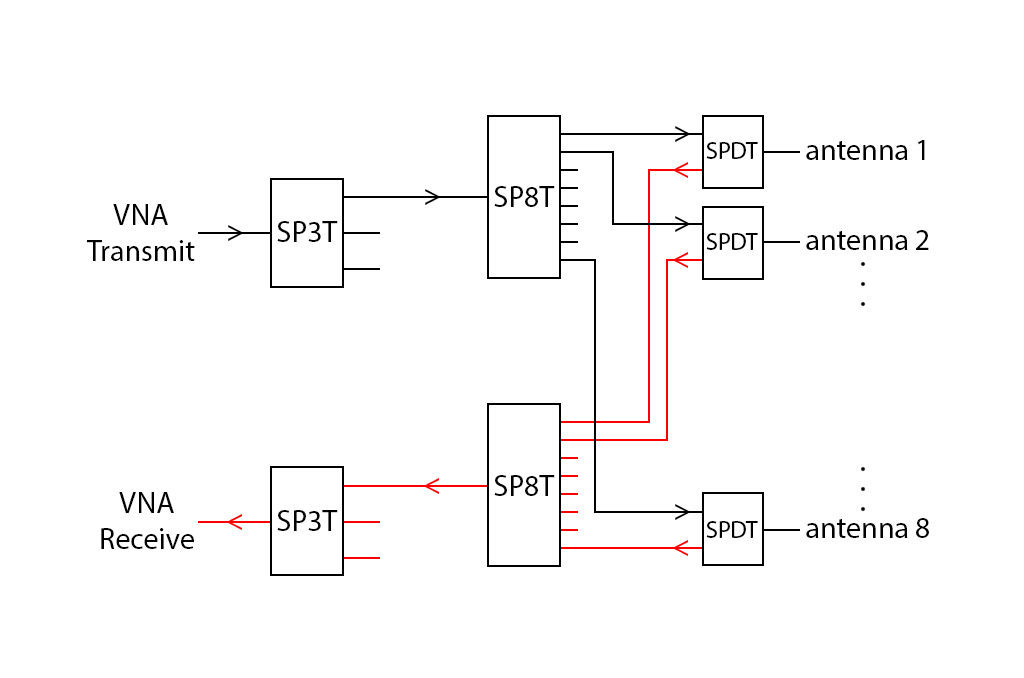
\includegraphics[width=5in]{./images/mp_final_layout.png}
		\caption{Final design of the multiplexer}
		\label{fig:mp_final_layout}
	\end{center}
\end{figure}


With this design decided on, we needed to get it manufactured on PCB. To create the PCB layout necessary to get these boards printed, software package Altium was used. Two boards were designed for the RF portion of the multiplexer; one containing only an SP3T and one containing two SP8Ts and eight SPDTs. The final 2 x 24 multiplexer requires two of the boards with SP3Ts and three of the boards with SP8Ts and SPDTs. The final PCB layout of the two boards is shown in figures \ref{fig:sp3t}, \ref{fig:sp8t_top} and \ref{fig:sp8t_bottom}.

Both boards were designed with 4 layers using a substrate of FR-4. The stack up of the boards consists of a top signal layer, followed by a substrate layer, then an internal signal layer (used only as ground in this design) and then the prepreg layer. Below the prepreg layer is a mirror of what is on top of it; an internal signal layer, then substrate layer and then bottom layer. The stack up from Altium is shown in figure \ref{fig:stackup}. 

Both boards used co-planar waveguides with ground for all of the RF traces and were designed such that they were 50 ohms. This resulted in a trace width of 0.5 mm and a gap of 0.115 mm with a substrate thickness of 0.6 mm. Three 10 pin connectors were added to provide power as well as connect all of the control pins for the SP8T and SPDT switches.

 
\begin{figure}[h]
	\begin{center}
		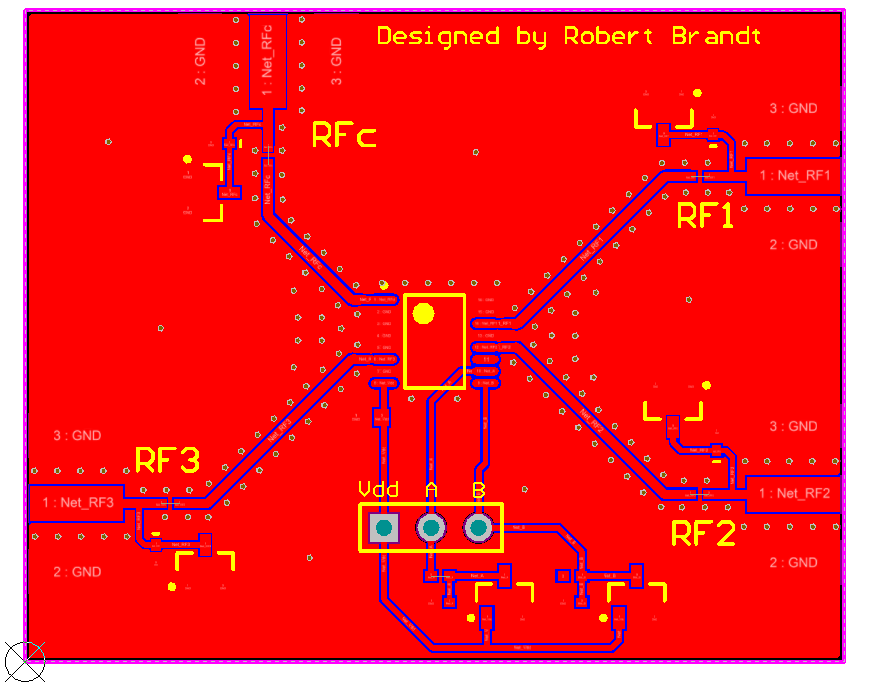
\includegraphics[width=3.5in]{./images/sp3t.png}
		\caption{PCB layout for SP3T board}
		\label{fig:sp3t}
	\end{center}
\end{figure}

\begin{figure}[h]
	\begin{center}
		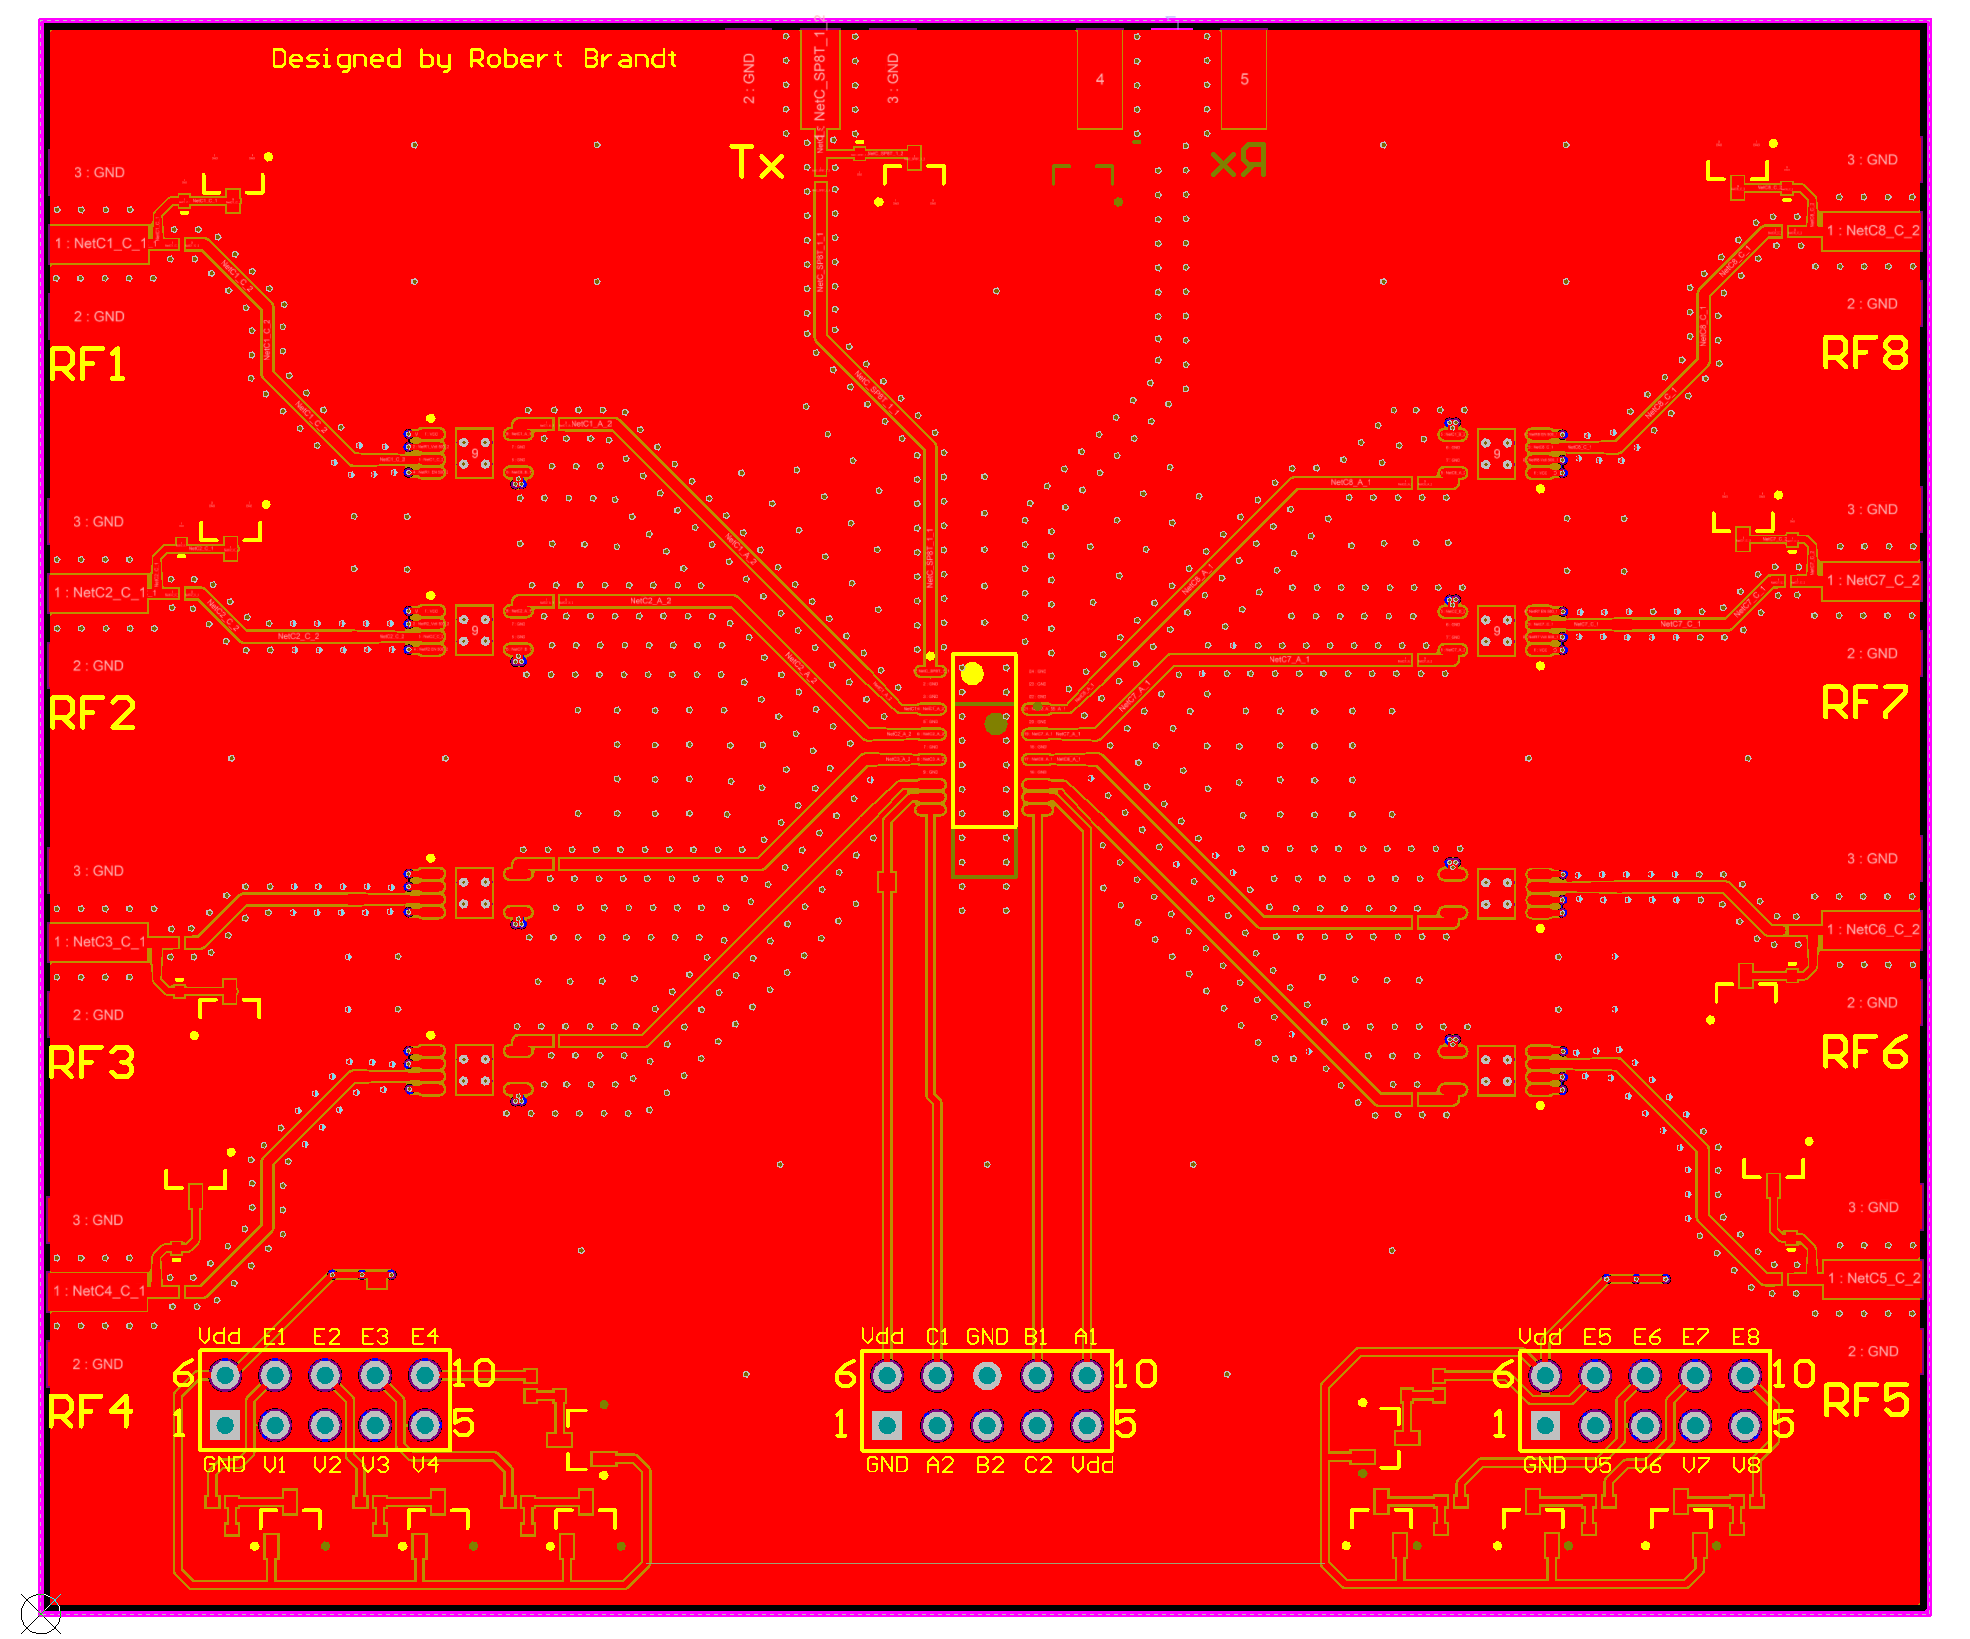
\includegraphics[width=5.5in]{./images/sp8t_top.png}
		\caption{PCB layout for top layer of SP8T and SPDT board}
		\label{fig:sp8t_top}
	\end{center}
\end{figure}

\begin{figure}[h]
	\begin{center}
		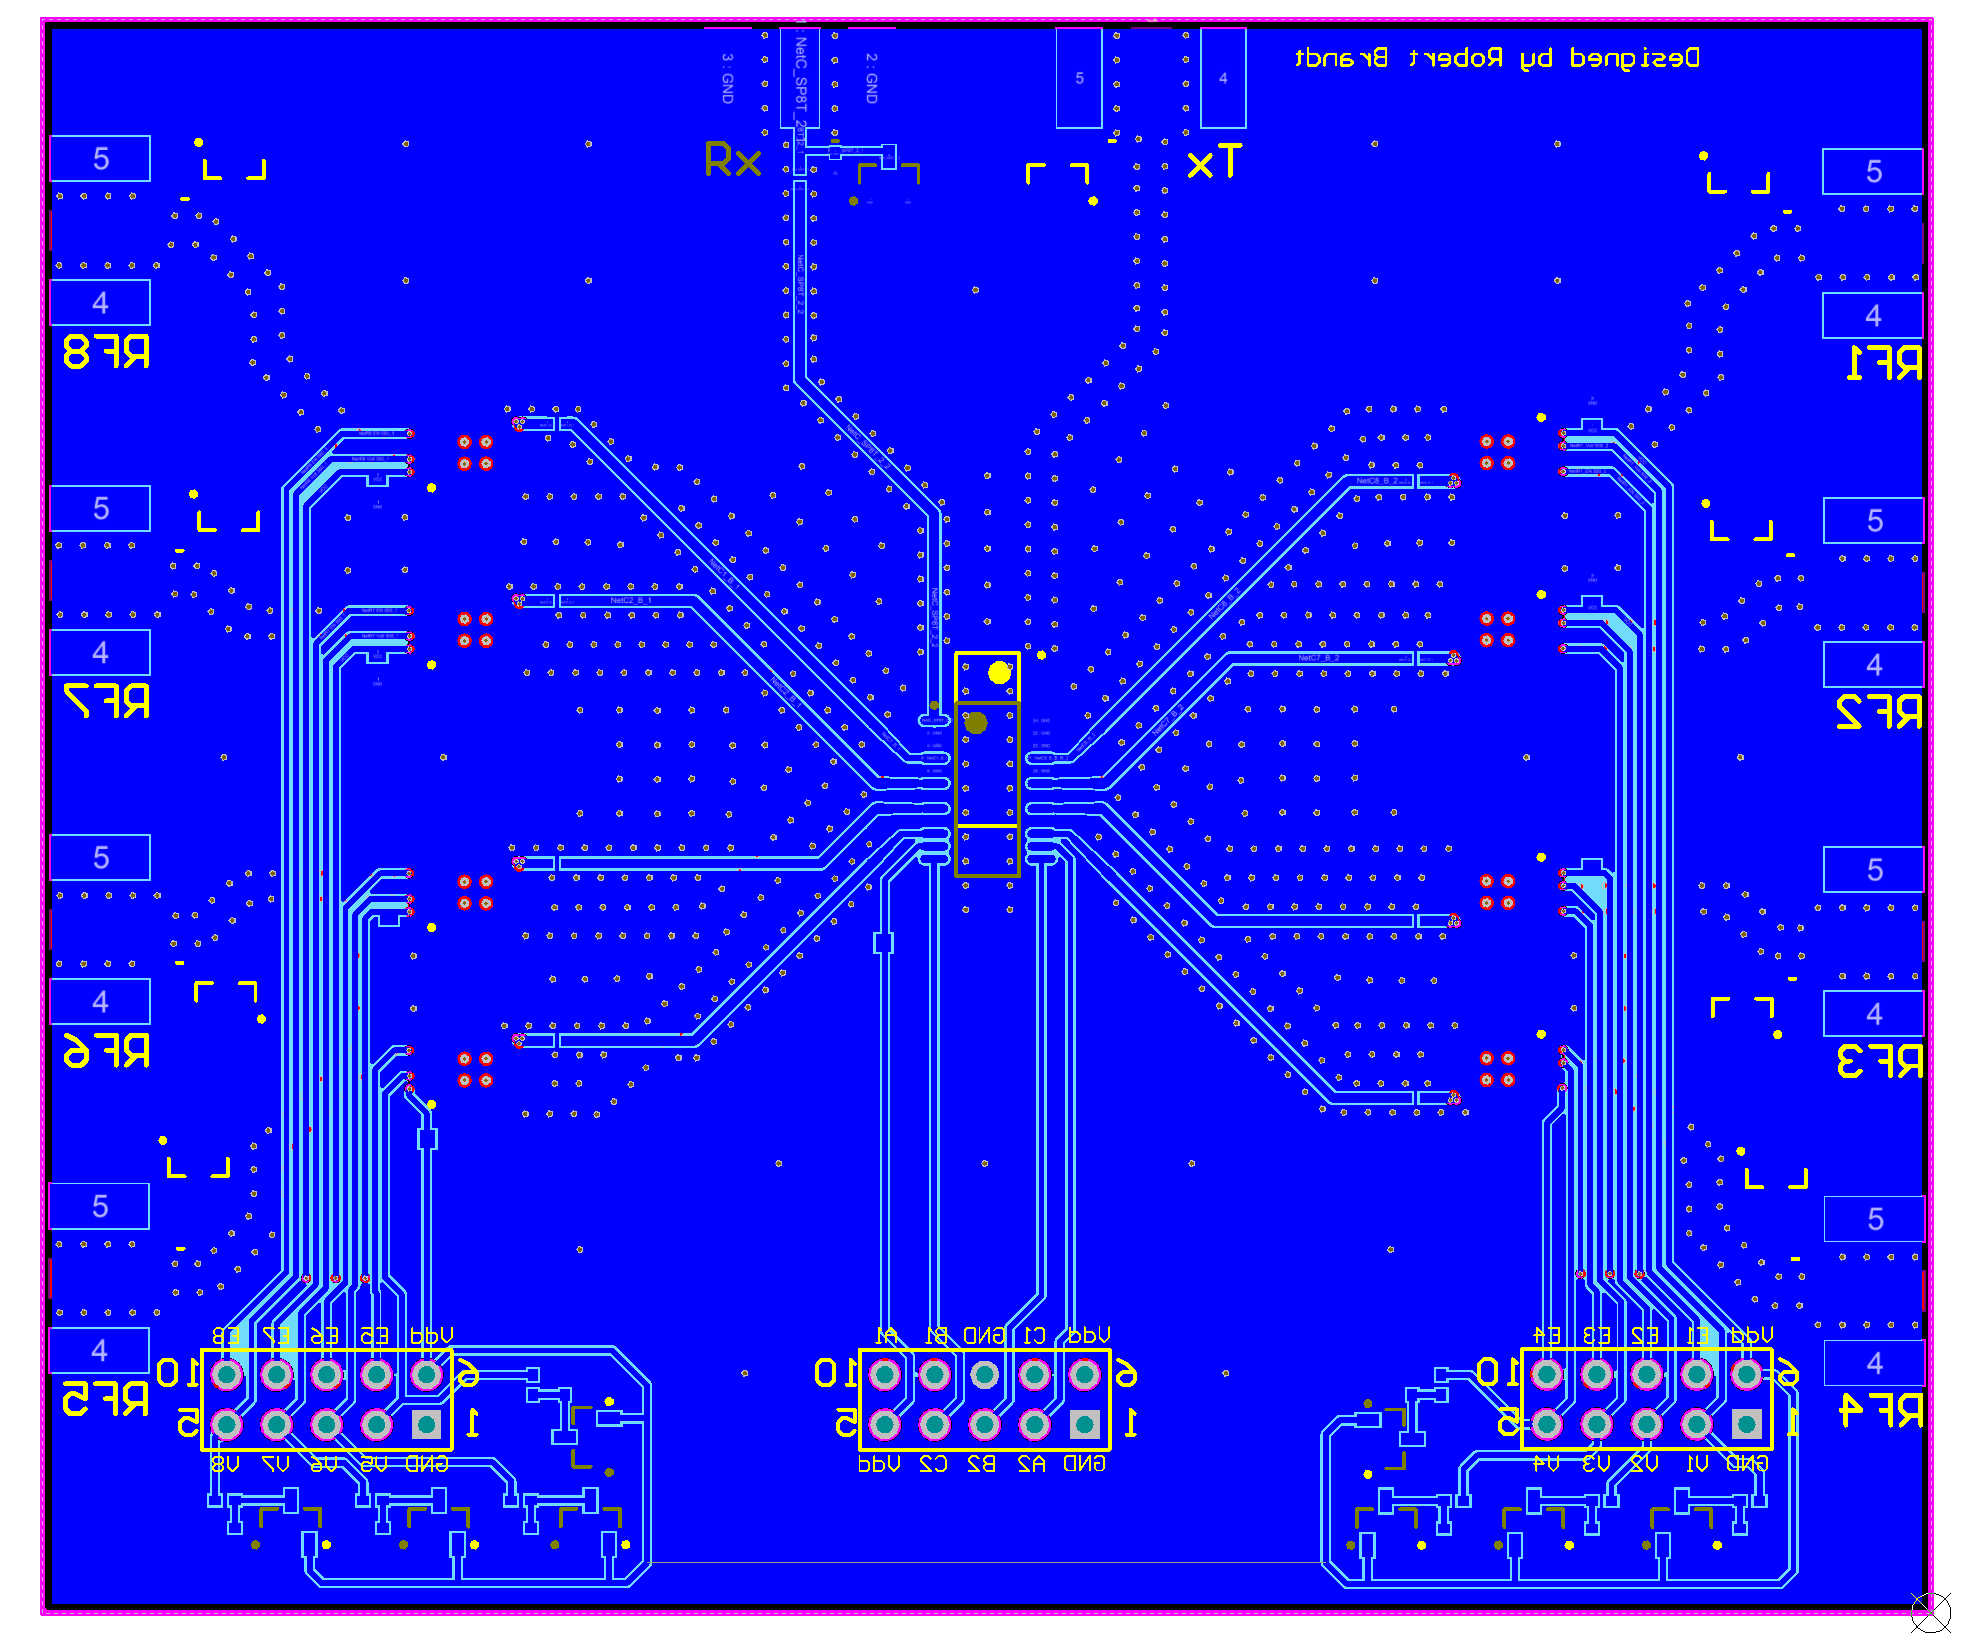
\includegraphics[width=5.5in]{./images/sp8t_bottom.png}
		\caption{PCB layout for bottom layer of SP8T and SPDT board}
		\label{fig:sp8t_bottom}
	\end{center}
\end{figure}

\begin{figure}[h]
	\begin{center}
		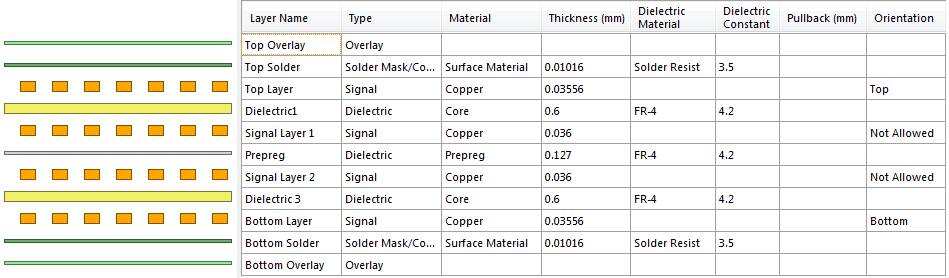
\includegraphics[width=5in]{./images/stackup.png}
		\caption{Stack up for PCBs in Altium}
		\label{fig:stackup}
	\end{center}
\end{figure}


Unfortunately, due to issues with our original intended supplier of our PCBs, we were unable to get these PCBs printed in time for this report. We found another supplier for our PCBs and hope to have them before our presentation. The PCBs needed to be modified somewhat due to different PCB specifications from this new supplier. Minimum routing size was larger at 0.1524 mm compared to 0.1 mm with the original supplier. Also, the substrate thickness options were different, not allowing us to use a thickness of 0.6 mm. Based on the specifications of the new supplier the RF traces needed to be modified to 0.185 mm thick with a gap of 0.1524 mm. This is based on a substrate thickness of 0.1 mm.


\section{DC Switching and Power Integration}

DC circuits are commonly used for controlling RF switches due to the cheaper cost in comparison to their RF counterparts and the reduction in frequency interference due to the maximum attenuation of any frequency components at DC. For our design we need a DC circuit for address decoding of the RF switch. In effect, the function of the DC switch is to set the control parameters in order to specify what the response of the RF switch will be at that point in time. 

\section{Research and Design}

\subsection{DC Switch}

At the onset of the project, we examined the previous switch design to understand how it would integrate with the RF switch and set the control parameters for the acquisition of data by the VNA. Our goal was to improve upon this design so that it was feasible with the new system we wanted to implement.

\subsection{Hardware}

The initial design appeared very complex and cumbersome to deduce because it had wires everywhere. The first task was therefore to ascertain the possibility of having a neater hardware with very minimal adjustment to the circuit after the printing of the PCB. This meant that most of the design should be implemented in the PCB in order to reduce complexity and make troubleshooting easier. This also ensure a reduction in noise cause by all the numerous wiring and addition electrical components that was everywhere.

The figure below highlights that function of the DC switch in perfect simplicity. The control parameters are letters from A – L and these are sourced from the DC switch to the SP3Ts, SP3Ts and SPDTs of the RF switch




\subsection{Software}

The software control of the DC switching circuit is done by an Arduino microcontroller loaded with a table that references the control lines for each multiplexer. This allows the SPDTs to function as an input or an output depending on the values set on the control lines but the Arduino. And will be concurrent with the presents action of the VNA such that, only one SPDT is in transmit mode at a given time. The software will also turn on one the SP8T for transmission of the signal and turn the other SP8Ts responsible for reception of the signals. 

After the research and understanding of requirements were satisfied, a truth table was drawn in order to simplify the circuit to its least possible scenario where the fewest components are used to achieve the expected results. This truth table was then transcribed into code for and then loaded unto the Arduino. This Arduino was set to function in synchronism with the raspberry pie.

\subsection{ESD Protection}

Any reliable system design requires some form of Electrostatic Discharge protection. Choosing the right circuit protection device involves considering criteria such as: Response time, ESD current handling capacity and, maximum reverse leakage current. Also the device should not interfere with the normal operation of the circuit. Designing the DC circuit also meant taking the RF circuit into consideration in order to minimize electrostatic discharge and current leakage. 

We considered N-well resisters, gate-grounded and gate-coupled protection options, silicon controlled rectifiers and diodes. Ultimately we decided to use diodes and capacitors due to its simplicity.

\subsection{Power Integration}

A portable power source will be integrated into our data collection unit to provide enough electrical power to run the VNA and the switch box simultaneously for the duration of time it takes to gather the parametric information from the VNA. 12V rechargeable battery which produces 3.0Ah of current will be hour choice as our power source.

\section{Design and Implementation}

\subsection{DC Switch}

The design of the switch required the use of Altium and the Arduino user interface. The hardware was designed in Altium and the software was writing in the Arduino mainframe in the C++ programing language 

\subsection{Hardware}

Designing the PCB first started with the schematic and a review of the schematic to ensure its accuracy. Below is the final schematic that was used in the printing of the PCB in Altium.









